\documentclass{article}

\usepackage{nips_2018}

\usepackage[T1]{fontenc}    % use 8-bit T1 fonts

% Useful packages
\usepackage{amsmath, amssymb, amsfonts, bm}
\usepackage{amsthm}
\usepackage{booktabs}       % professional-quality tables
\usepackage{mathtools}
\usepackage{nicefrac}       % compact symbols for 1/2, etc.
\usepackage[usenames, dvipsnames]{color}
\usepackage{multirow}
\usepackage{hyperref}

\usepackage{floatrow}
\floatsetup[table]{capposition=top}

\usepackage{wrapfig}
\usepackage{multicol}

\setlength{\columnsep}{1cm}
\setlength{\columnseprule}{0.5pt}
\def\columnseprulecolor{\color{Plum}}

% Simple macros.
\def\sec#1{Sec.~\ref{#1}}
\def\Sec#1{Sec.~\ref{#1}}
\def\fig#1{Fig.~\ref{#1}}
\def\Fig#1{Fig.~\ref{#1}}
\def\tableref#1{Table~\ref{#1}}

\newcommand{\tk}[1]{\textcolor{red}{TK: #1}}
\newcommand{\tkf}[1]{\footnote{\tk{#1}}}
\newcommand{\ao}[1]{\textcolor{green}{AO: #1}}
\newcommand{\tsj}[1]{\textcolor{magenta}{TSJ: #1}}
\newcommand{\vm}[1]{\textcolor{blue}{Vincent M: #1}}
\newcommand{\vmf}[1]{\footnote{\vm{#1}}}


\newcommand{\cw}{\mathbf{cw}}
\newcommand{\cc}{\mathbf{c}}
\newcommand{\kb}{\mathbf{k}}
\newcommand{\mem}{\mathbf{m}}
\newcommand{\rr}{\mathbf{r}}

\title{On the performance of the MAC model}

% The \author macro works with any number of authors. There are two
% commands used to separate the names and addresses of multiple
% authors: \And and \AND.
%
% Using \And between authors leaves it to LaTeX to determine where to
% break the lines. Using \AND forces a line break at that point. So,
% if LaTeX puts 3 of 4 authors names on the first line, and the last
% on the second line, try using \AND instead of \And before the third
% author name.

\author{}
%\author{
%  MI-Prometheus\thanks{%
%  It's scary --- \href{https://www.imdb.com/title/tt1446714/}{and it's back!}} \\
%  %% examples of more authors
%  %% \And
%  %% Coauthor \\
%  %% Affiliation \\
%  %% Address \\
%  %% \texttt{email} \\
%  %% \AND
%  %% Coauthor \\
%  %% Affiliation \\
%  %% Address \\
%  %% \texttt{email} \\
%  %% \And
%  %% Coauthor \\
%  %% Affiliation \\
%  %% Address \\
%  %% \texttt{email} \\
%  %% \And
%  %% Coauthor \\
%  %% Affiliation \\
%  %% Address \\
%  %% \texttt{email} \\
%}

\begin{document}
% \nipsfinalcopy is no longer used

\maketitle

\begin{abstract}
  The abstract paragraph should be indented \nicefrac{1}{2}~inch
  (3~picas) on both the left- and right-hand margins. Use 10~point
  type, with a vertical spacing (leading) of 11~points.  The word
  \textbf{Abstract} must be centered, bold, and in point size 12. Two
  line spaces precede the abstract. The abstract must be limited to
  one paragraph.
\end{abstract}
\section{Introduction}
Reasoning over visual inputs is a fundamental characteristic of human intelligence.
Reproducing this ability with artificial agents is a challenge that requires learning relations and compositionality (Hu et al. 2017; Johnson et al. 2017b).

The Visual Question Answering (VQA) task has been tailored to benchmark those reasoning performances. It is a complex semantic task requiring both natural language processing and visual recognition. It also puts to the test the effective use of the short term memory.

The recent CLEVR dataset (Johnson et al., 2017a) proposes a challenging multimodal task that requires to answer compositional questions about an image. The dataset is designed with the explicit goal of enabling detailed analysis of visual reasoning.
Solving this problem involves a broad array of skills such as counting, comparison and understanding transitive reasoning.
It also requires perceptual abilities such as recognizing objects, attributes, and spatial relations as well as leveraging commonsense world knowledge (Hudson et al. 2018).
CLEVR is a generated synthetic dataset that allows to introduce variations on a subset of data to test a particular ability such as generalization or transfer learning.

To solve this type of reasoning task, many deep learning approaches have been explored although they often struggle to perform well on tasks with a structured and compositional nature (Garnelo et al., 2016; Lake et al., 2017). 
More recent approaches adopt modular structures, resembling the trees of programming languages, that compose neural modules from a fixed predefined collection (Andreas et al., 2016a; Johnson et al., 2017b, Mascharka et al., 2018). However, they rely on externally provided structured representations and functional programs, parsers or expert demonstration, and sometimes require reinforcement learning training schemes (Hudson et al. 2018). 
These models’ structure is inherently rigid and the use of a range of specialized modules weaken their robustness and generalization capacities.

Recent work on CLEVR from Hudson et al. 2018;  has introduced  MAC ( Memory, Attention, and Composition). The MAC model has been deliberately designed to decompose the problem into a sequence of attention-based reasoning operations. Its ability to arbitrarily draw a complex reasoning graph while still featuring end-to-end differentiability made its sucess.
MAC doesn’t use specific modules that would make it specifically tailored for the CLEVR dataset. The three general units working in tandem to perform a reasoning step make the robustness of the model.

MAC achieves state-of-the-art accuracy on CLEVR and also on the most difficult CLEVR Humans dataset, were questions are written by humans. 
Although the performance of MAC has been proven, It appears difficult to understand what concepts the model is learning. 
Does the model really learn relations between objects? 
How does the model represent those relations and reasoning steps? 
The interpretability of the MAC model seems yet to be fully defined.
Is the model representing notions and concepts like objects attributes?

In this work, we first question the complexity of the MAC model and explore simplification possibilities. We propose a new set of equations that aims to simplify the model and improve training performance. 
We also put to proof the MAC model on the CLEVR CoGenT dataset. The CoGenT dataset has been designed to highlight transfer learning abilities and give a better sense of interpretability. By mixing attributes over two sub-datasets, the CLEVR CoGenT task allow us to see what relations and concepts the model has really learned. We show how MAC performs on CLEVR CoGenT and compare it to state-of-the-art models and propose a study about the model failures. This work points out some of the MAC model weaknesses, in particular its failure to differentiate concepts of colors and shape. We finally discuss some improvement possibilities.

\section{Description of MAC model}


A MAC network is an end-to-end differentiable architecture primed to perform an explicit multi-step reasoning process, by stringing together p recurrent MAC cells, each responsible for performing one reasoning step. Given a knowledge base K (for VQA, an image) and a task description q (for VQA, a question), the model infers a decomposition into a series of p reasoning operations that interact with the knowledge base, iteratively aggregating and manipulating information to perform the task at hand. It consists of three components: (1) an input unit, (2) the core recurrent network, composed out of p MAC cells, and (3) an output unit, all described below.

\begin{figure}[htbp]
	\centering
	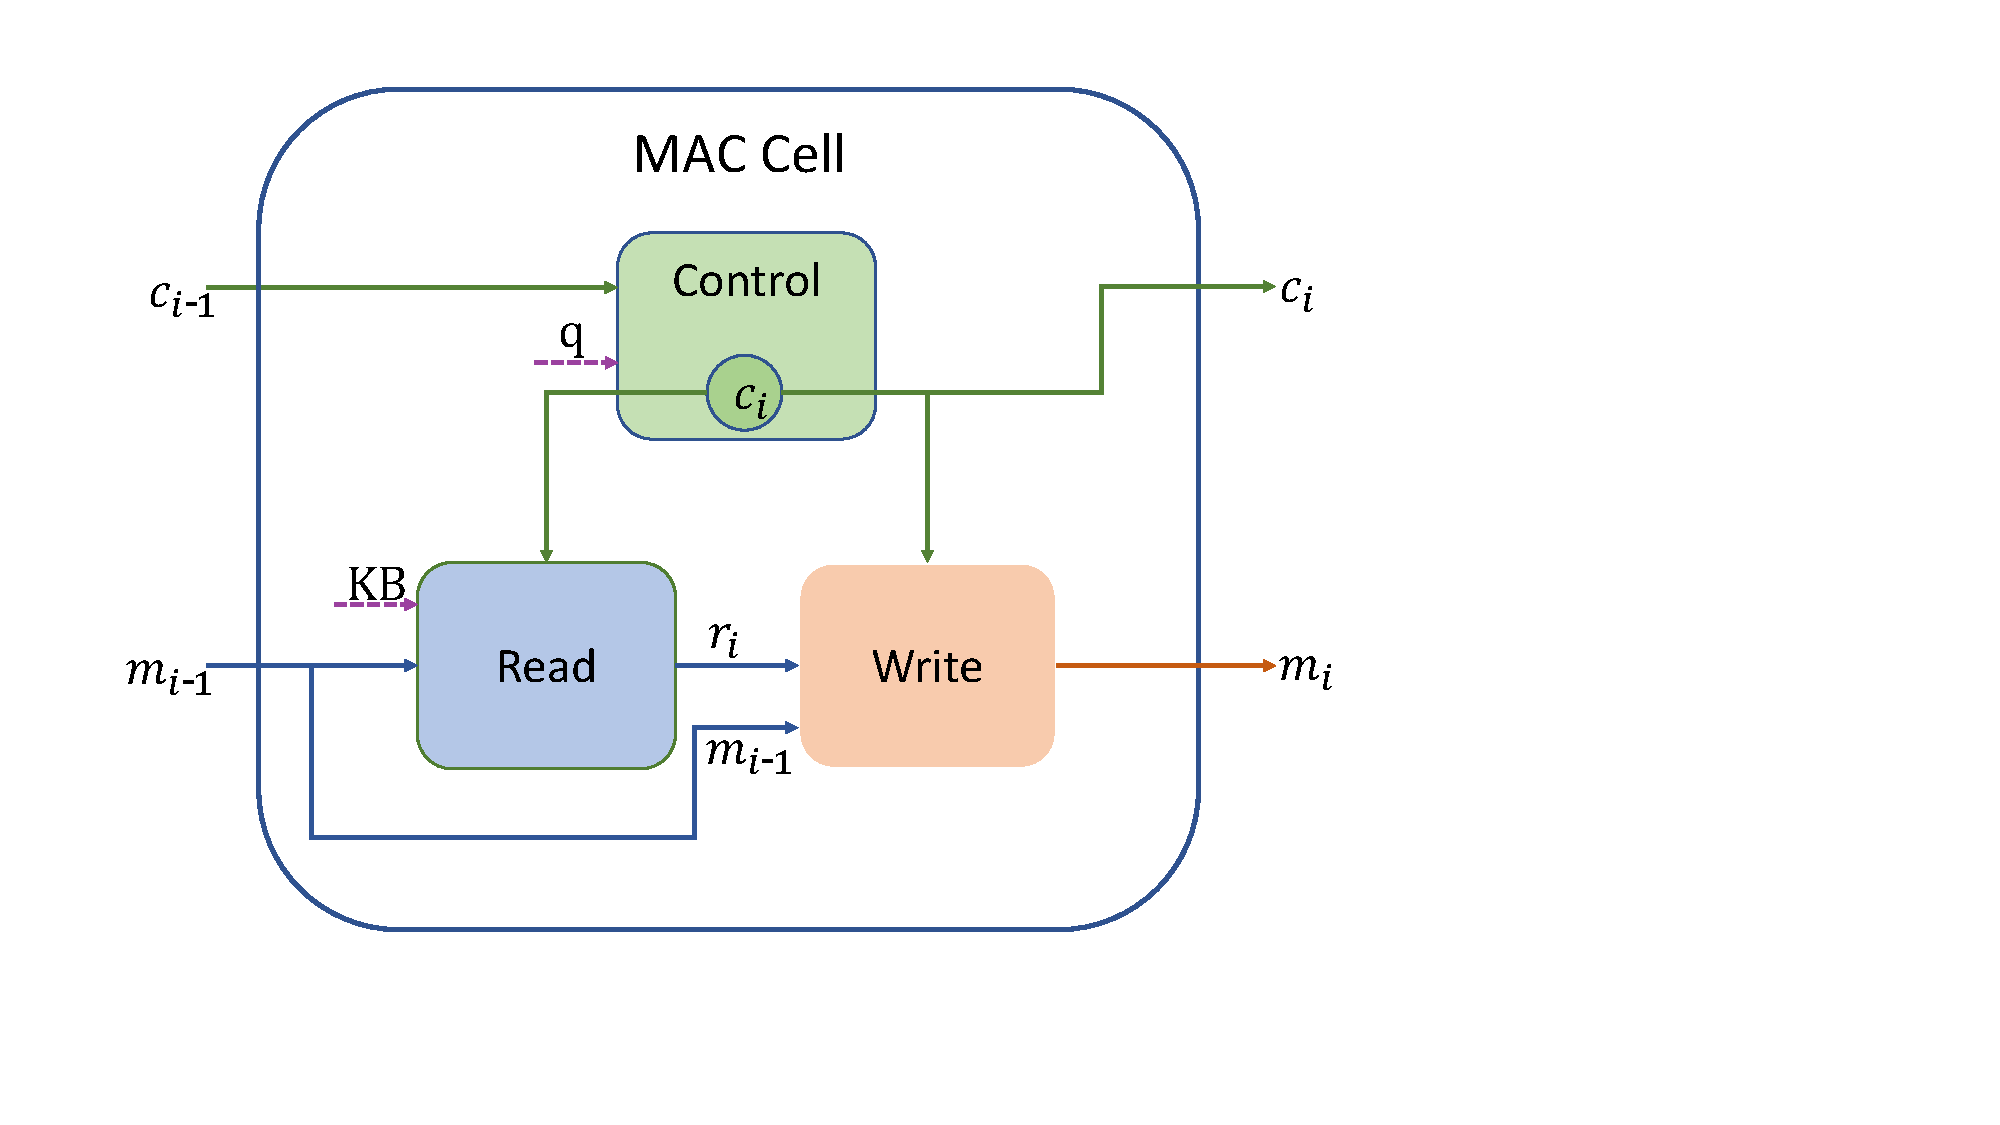
\includegraphics[width=0.7\textwidth]{img/mac_cell.pdf}
	\caption{The Mac Cell. The MAC recurrent cell consists of a control unit, read unit, and write unit, that operate over dual control and memory hidden states. The control unit successively attends to different parts of the task description (question), updating the control state to represent at each timestep the reasoning operation the cell intends to perform. The read unit extracts information out of a knowledge base (here, image), guided by the control state. The write unit integrates the retrieved information into the memory state, yielding the new intermediate result that follows from applying the current reasoning operation.}
	\label{fig:core_concepts}
\end{figure}


\subsection{Simplified MAC network}
Our proposed modification to the MAC network is based on two heuristic
simplifications of the equations governing a MAC cell. 
First, we observed that when looking at the equations of different units
together as a whole, we notice that there are several affine transformations
that are applied in sequence (with no activation in-between).
Therefore they can actually be combined to form a single affine transformation.
The second observation uses the following heuristic argument:
suppose there is a single affine transformation which preserves the number
of dimensions. Then one can assume that the transformation is invertible
so as to avoid a loss in the information. Applying this principle to 
equations in the read and write unit results in eliminating an affine
operation of the knowledge base in the recurrent network. Instead we compute
this operation on the knowledge base right after we apply the 2 
trainable CNN layers (i.e. prior to the reasoning steps). This results
in a significant savings in training time, as our experiments demonstrate
below, without incurring too much drop in accuracy.

In the description below, the original MAC cell equations are shown on the \emph{left}
while our simplified equations are shown (in color) on the {\color{Plum} \emph{right}}.
(The equation numbering is the same as in~\cite{hudson2018compositional}.)

\noindent\textit{Notation:} The index/position $i$ below denotes the reasoning step. 
Unless mentioned otherwise, the weights/biases are invariant w.r.t $i$, 
i.e., shared across all the reasoning steps. 

\noindent\textbf{Control unit:} 
For both models, in the control unit, the question $q$ is first transformed in each step of 
%the reasoning using a \emph{position-aware}~\cite{hudson2018compositional} 
linear layer: $q_i = U_i^{[d \times 2d]} q + b_i^{[d]}$.

\begin{multicols}{2}
	\noindent
	\begin{align*}
	&cq_i = W_{cq}^{[d \times 2d]} [c_{i-1}, q_i] + b_{cq}^{[d]}  \tag{c1} \\
	&ca_{is} = W_{ca}^{[1 \times d]} (cq_i \odot \cw_s) + b_{ca}^{[1]}
	\tag{c2.1}\\
	&cv_{is} = \textrm{softmax}(ca_{is}) \tag{c2.2}\\
	&\cc_i = \sum_s cv_{is} \, \cw_s  \tag{c2.3}
	\end{align*}
	\columnbreak
	{\color{Plum}
	\begin{align*}
	&cq_i = W_{cq}^{[d \times d]} c_{i-1} + q_i  \tag{c1} \\
	&ca_{is} = W_{ca}^{[1 \times d]} (cq_i \odot \cw_s)  \tag{c2.1}\\
	&cv_{is} = \textrm{softmax}(ca_{is}) \tag{c2.2}\\
	&\cc_i = \sum_s cv_{is} \, \cw_s  \tag{c2.3}
    \end{align*}}
\end{multicols}

\noindent\textbf{Read and write units:}
For both models below, $\kb_{hw}$ denotes the 
\emph{knowledge base}~\cite{hudson2018compositional}
consisting of 3D tensors with dimension $H \times W \times d$ for each image
in the data set. The difference in computing $\kb_{hw}$ is that the simplified MAC uses
an additional linear layer on top of the 2 CNN layers present in the original MAC network.
This circumvents the need for performing additional linear transformations on the 
knowledge base, as is done by the original MAC network in \emph{each} reasoning step.

\begin{multicols}{2}
	\noindent
	\begin{align*}
	&I_{ihw} = (W_{m}^{[d \times d]} \mem_{i-1} + b_{m}^{[d]}) \\
	           & \qquad \quad \odot (W_{k}^{[d \times d]} \kb_{hw} + b_{k}^{[d]}) \tag{r1} \\
	&I'_{ihw} =  W_{I'}^{[d \times 2d]} [I_{ihw},\kb_{hw}]  + b_{I'}^{[d]}  \tag{r2} \\
	&ra_{ihw} = W_{ra}^{[1 \times d]} (\cc_i \odot I'_{ihw}) + b_{ra}^{[1]} \tag{r3.1}\\
	&rv_{ihw} = \textrm{softmax}(ra_{ihw}) \tag{r3.2}\\
	&\rr_i = \sum_s rv_{ihw} \, \kb_{hw}  \tag{r3.3}\\
	&\mem_i = W_{rm}^{[d \times d]} [\rr_i, \mem_{i-1}]  + b_{rm}^{[d]} \tag{w1}	
	\end{align*}
	\columnbreak
	{\color{Plum}
	\begin{align*}
	&I_{ihw} = \mem_{i-1} \odot \kb_{hw} \tag{r1} \\ \\
	&I'_{ihw} = W_{I'}^{[d \times d]} I_{ihw} + b_{I'}^{[d]} + \kb_{hw} \tag{r2} \\
	&ra_{ihw} = W_{ra}^{[1 \times d]} (\cc_i \odot I'_{ihw})  \tag{r3.1}\\
	&rv_{ihw} = \textrm{softmax}(ra_{ihw}) \tag{r3.2}\\
	&\rr_i = \sum_s rv_{ihw} \, \kb_{hw}  \tag{r3.3}\\
	&\mem_i = W_{rm}^{[d \times d]} \rr_i + b_{rm}^{[d]} \tag{w1}
	\end{align*}}
\end{multicols}


\section{Experiments}

We evaluated SAMNet on the COG dataset~\cite{yang2018dataset}.
Our experiments were designed to study SAMNet's performance as well as its generalization abilities in different settings.
For this purpose, we used two different variants of the COG dataset: an easy one (Canonical) and a Hard version to explore a wide range of difficulties.
The main differences are the number of frames in the input sequence (4 vs. 8) and the maximum number of distractors (i.e., objects not relevant for the answer) per frame (1 vs. 10).
%More details on the dataset, its variants and tasks can be found in the Appendix.


%
%We compare our model to the original COG model  ~\cite{yang2018dataset} using their implementation (https://github.com/google/cog) and scores given by the authors. We also use the exact same training parameters detailed in the original paper.
%
%On the other side we trained SAMNet using IBM's Mi-Prometheus~\cite{kornuta2018accelerating}, a framework for research based on Pytorch. We trained all our models using NVIDIA’s GeForce GTX TITAN X GPUs. We trained  SAMNet using 8 reasoning steps SAMCells and a hidden state size of 128. The external memory has 128-bit slots. We trained our model until convergence but we also have set a training time limit of 80 hours.


\begin{figure}[htbp]
	\centering
  \begin{subfigure}{\textwidth}
    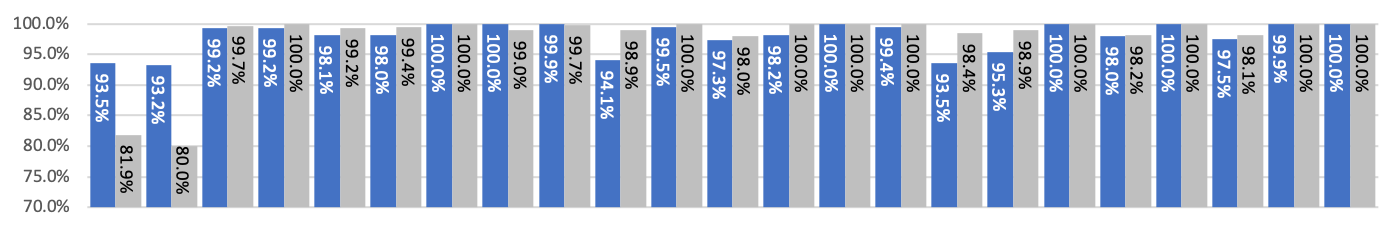
\includegraphics[width=0.92\textwidth]{../results/samnet_cog_orig_canonical_no_labels.png}
  \end{subfigure}%
  \newline
  \begin{subfigure}{\textwidth}
	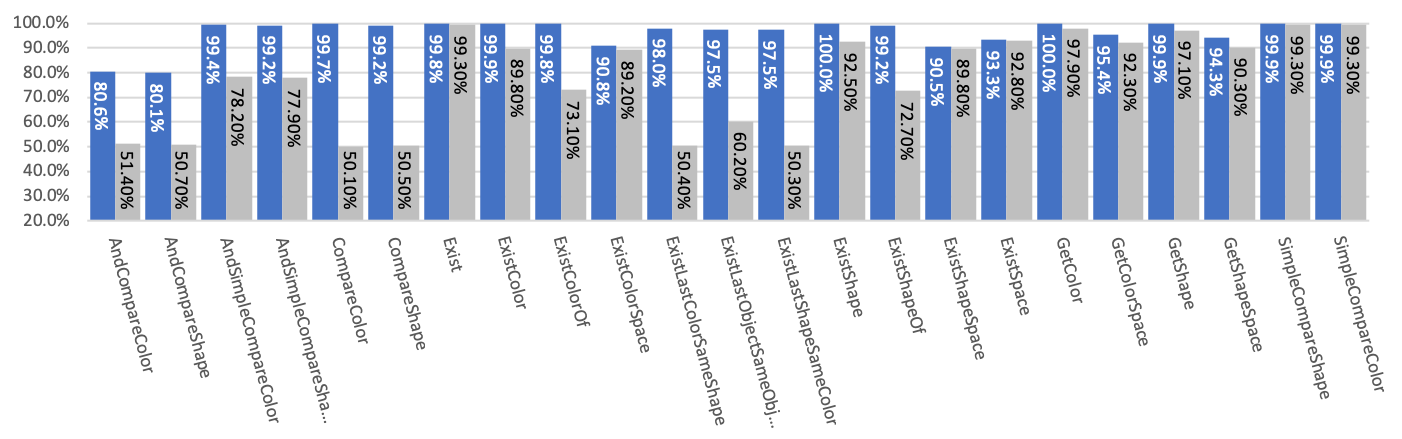
\includegraphics[width=0.93\textwidth]{../results/samnet_cog_orig_hard.png}
  \end{subfigure}%
\caption{Comparison of test set accuracies of SAMNet (blue) with original results achieved by the COG model (gray) on Canonical (top) and Hard (bottom) variants of the COG dataset.}
\label{fig:samnet_cog_detailed}
\end{figure}

\begin{figure}
	\centering
	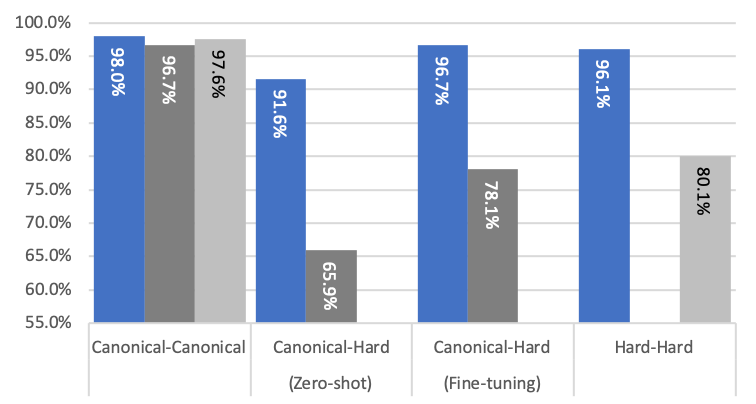
\includegraphics[width=0.75\textwidth]{../results/samnet_cog_overall_transfer.png}
	\caption{Total accuracies of SAMNet (blue) and COG models (light/dark gray) when testing generalization from Canonical to Hard variants of the dataset.}
	\label{fig:samnet_cog_overall_transfer}
\end{figure}

We have implemented and trained our SAMNet model using MI-Prometheus~\cite{kornuta2018accelerating}, a framework based on Pytorch~\cite{paszke2017automatic}. 
In our experiments, we have focused on 22 classification tasks and compared our results with the baseline model, as presented in \cref{fig:samnet_cog_detailed}.
For the Canonical variant (top row), we have achieved similar accuracies for the majority of tasks (with the total average accuracy of 98.0\% in comparison of 97.6\% achieved by the COG model), with significant improvements (around 13 points) for \textit{AndCompare} tasks.
As those tasks focus on compositional questions referring to two objects, we hypothesize that our model achieved better accuracy due to the ability to selectively pick and store the relevant objects from the past frames in the memory.
Despite there being some tasks in which our model reached slightly lower accuracies,
% (between 0.2 and 1.8 points)
when comparing performances on the Hard variant, it improves upon the  COG baseline on all tasks, with improvements varying from 0.5 to more than 30 points.

The goal of the next set of experiments was to test the generalization ability concerning the sequence length and number of distractors.
For that purpose, we have compared the accuracies of both models when trained on the Canonical variant and tested on Hard (\cref{fig:samnet_cog_overall_transfer}).
As the original paper does not include such experiments, we have performed them on our own.  The light gray color indicates the original results, whereas dark gray indicates the accuracies of COG models that we have trained (fine-tuning/testing) using the original code provided by the authors.
For sanity check, in the first column, we report both the best-achieved score and the score reported in the paper when training and testing on Canonical variant, without any fine-tuning.
In a pure \textit{transfer learning} setup (second column), our model shows enormous generalization ability, reaching 91.6\% accuracy on the test set.
We have also tested both models in a setup where the model trained on a Canonical variant underwent additional fine-tuning (for a single epoch) on the Hard variant (third column).
In this case, the SAMNet model also reached much better performance, and, interestingly, achieved better scores from the model trained and tested exclusively on the Hard variant.
In summary, the results clearly indicate that the mechanisms introduced in SAMNet  enable it to learn to operate independently of the total number of frames or number of distractions, and allow it to generalize to longer videos and more complex scenes. One other strength of SAMNet is its interpretability. Observing attention maps (see supplementary material) shows that SAMNet can effectively perform multi-step reasoning over questions and frames as intended. It also accurately classifies temporal contexts as designed. However we notice that the model can sometime discover alternative strategies that were not in the intended design but the answers are still correct. 

%we used the canonical (easy) and hard settings that alter the number of distractors and sequence length.  Since there was no baseline for these tests (train on canonical, test on hard), we ran our own experiments using the COG model provided by the authors.  SAMNet achieves the highest overall scores for all categories of experiments (\cref{fig:samnet_cog_overall_transfer}), especially for the tests run on the hard dataset.  Among the 22 classification tasks, we highlighted the two most difficult tasks that affect the overall score. 
%We argue that the generalization capability of SAMNet is mainly due to the dynamic frame-by-frame processing of the input sequence. 
%The mechanisms introduced in SAMCell learn to operate independently of the total number of frames and allow to generalize to longer video lengths.
%As shown in \cref{fig:samnet_cog_overall_transfer}, when trained on the easy dataset, SAMNet still performs 91.6\% when tested on the hard dataset, whereas COG drops from 97.6\% to 65.9\%   The visualization of the trained SAMNet model (see Appendix) indicates that the model learns the concept of time, helping it to control the flow of information from visual input to the memory.  Therefore, the memory is updated efficiently instead of storing all information across all frames.






\section{Conclusion}


\bibliographystyle{alpha}
\bibliography{vigil_bibliography}

\end{document}
